% **** Szablon pracy magisterskiej, licencjackiej lub inżynierskiej ****

\documentclass[polish,12pt,twoside,a4paper]{report}

% *************** Definicje stylu dokumentu ***************

% *********************************************************************************
% W pliku tym zdefiniowany jest wygl¹d dokumentu.
% Zmiany tutaj nie s¹ konieczne o ile nie zamierzasz zmieniaæ wygl¹du dokumentu.
% *********************************************************************************

% *************** Za³adowanie pakietów ***************
\usepackage[a4paper,twoside,left=2.0cm,right=1.5cm,top=1.5cm,bottom=1.5cm]{geometry}
\usepackage[T1]{fontenc}
%\usepackage[cp1250]{inputenc}
\usepackage[utf8]{inputenc}
\usepackage[polish]{babel}
\usepackage{amsmath}
\usepackage{amsfonts}
\usepackage{graphicx}
\usepackage{graphics}
\usepackage{times}
\usepackage{indentfirst}%wciecia a nowych akapitach
\usepackage{listings}
\usepackage{url}
\usepackage[colorlinks=true, linkcolor=black, urlcolor=black, citecolor=black]{hyperref}

\selectlanguage{polish}

%szerokoœœ wciêæ
\setlength{\parindent}{1.25cm}

%numeracja stron
\usepackage{fancyhdr}
\pagestyle{fancy}
\fancyhf{} % usun biezace ustawienia pagin
\fancyhead[LE,RO]{ }
\fancyhead[LO]{ }
\fancyhead[RE]{ }
\fancyfoot[LE,RO]{\small\thepage}
\fancyfoot[LO]{ }
\fancyfoot[RE]{ }
\renewcommand{\headrulewidth}{0.0pt}
\renewcommand{\footrulewidth}{0.0pt}
\addtolength{\headheight}{0.0pt} % pionowy odstep na kreske
\fancypagestyle{plain}{%
\fancyhead{} % usun p. górne na stronach pozbawionych
% numeracji (plain)
\renewcommand{\headrulewidth}{0.0pt} % pozioma kreska
}

% *************** Definicje niektórych kolorów ***************
\usepackage{color}

\definecolor{greenyellow}   {cmyk}{0.15, 0   , 0.69, 0   }
\definecolor{yellow}        {cmyk}{0   , 0   , 1   , 0   }
\definecolor{goldenrod}     {cmyk}{0   , 0.10, 0.84, 0   }
\definecolor{dandelion}     {cmyk}{0   , 0.29, 0.84, 0   }
\definecolor{apricot}       {cmyk}{0   , 0.32, 0.52, 0   }
\definecolor{peach}         {cmyk}{0   , 0.50, 0.70, 0   }
\definecolor{melon}         {cmyk}{0   , 0.46, 0.50, 0   }
\definecolor{yelloworange}  {cmyk}{0   , 0.42, 1   , 0   }
\definecolor{orange}        {cmyk}{0   , 0.61, 0.87, 0   }
\definecolor{burntorange}   {cmyk}{0   , 0.51, 1   , 0   }
\definecolor{bittersweet}   {cmyk}{0   , 0.75, 1   , 0.24}
\definecolor{redorange}     {cmyk}{0   , 0.77, 0.87, 0   }
\definecolor{mahogany}      {cmyk}{0   , 0.85, 0.87, 0.35}
\definecolor{maroon}        {cmyk}{0   , 0.87, 0.68, 0.32}
\definecolor{brickred}      {cmyk}{0   , 0.89, 0.94, 0.28}
\definecolor{red}           {cmyk}{0   , 1   , 1   , 0   }
\definecolor{orangered}     {cmyk}{0   , 1   , 0.50, 0   }
\definecolor{rubinered}     {cmyk}{0   , 1   , 0.13, 0   }
\definecolor{wildstrawberry}{cmyk}{0   , 0.96, 0.39, 0   }
\definecolor{salmon}        {cmyk}{0   , 0.53, 0.38, 0   }
\definecolor{carnationpink} {cmyk}{0   , 0.63, 0   , 0   }
\definecolor{magenta}       {cmyk}{0   , 1   , 0   , 0   }
\definecolor{violetred}     {cmyk}{0   , 0.81, 0   , 0   }
\definecolor{rhodamine}     {cmyk}{0   , 0.82, 0   , 0   }
\definecolor{mulberry}      {cmyk}{0.34, 0.90, 0   , 0.02}
\definecolor{redviolet}     {cmyk}{0.07, 0.90, 0   , 0.34}
\definecolor{fuchsia}       {cmyk}{0.47, 0.91, 0   , 0.08}
\definecolor{lavender}      {cmyk}{0   , 0.48, 0   , 0   }
\definecolor{thistle}       {cmyk}{0.12, 0.59, 0   , 0   }
\definecolor{orchid}        {cmyk}{0.32, 0.64, 0   , 0   }
\definecolor{darkorchid}    {cmyk}{0.40, 0.80, 0.20, 0   }
\definecolor{purple}        {cmyk}{0.45, 0.86, 0   , 0   }
\definecolor{plum}          {cmyk}{0.50, 1   , 0   , 0   }
\definecolor{violet}        {cmyk}{0.79, 0.88, 0   , 0   }
\definecolor{royalpurple}   {cmyk}{0.75, 0.90, 0   , 0   }
\definecolor{blueviolet}    {cmyk}{0.86, 0.91, 0   , 0.04}
\definecolor{periwinkle}    {cmyk}{0.57, 0.55, 0   , 0   }
\definecolor{cadetblue}     {cmyk}{0.62, 0.57, 0.23, 0   }
\definecolor{cornflowerblue}{cmyk}{0.65, 0.13, 0   , 0   }
\definecolor{midnightblue}  {cmyk}{0.98, 0.13, 0   , 0.43}
\definecolor{navyblue}      {cmyk}{0.94, 0.54, 0   , 0   }
\definecolor{royalblue}     {cmyk}{1   , 0.50, 0   , 0   }
\definecolor{blue}          {cmyk}{1   , 1   , 0   , 0   }
\definecolor{cerulean}      {cmyk}{0.94, 0.11, 0   , 0   }
\definecolor{cyan}          {cmyk}{1   , 0   , 0   , 0   }
\definecolor{processblue}   {cmyk}{0.96, 0   , 0   , 0   }
\definecolor{skyblue}       {cmyk}{0.62, 0   , 0.12, 0   }
\definecolor{turquoise}     {cmyk}{0.85, 0   , 0.20, 0   }
\definecolor{tealblue}      {cmyk}{0.86, 0   , 0.34, 0.02}
\definecolor{aquamarine}    {cmyk}{0.82, 0   , 0.30, 0   }
\definecolor{bluegreen}     {cmyk}{0.85, 0   , 0.33, 0   }
\definecolor{emerald}       {cmyk}{1   , 0   , 0.50, 0   }
\definecolor{junglegreen}   {cmyk}{0.99, 0   , 0.52, 0   }
\definecolor{seagreen}      {cmyk}{0.69, 0   , 0.50, 0   }
\definecolor{green}         {cmyk}{1   , 0   , 1   , 0   }
\definecolor{forestgreen}   {cmyk}{0.91, 0   , 0.88, 0.12}
\definecolor{pinegreen}     {cmyk}{0.92, 0   , 0.59, 0.25}
\definecolor{limegreen}     {cmyk}{0.50, 0   , 1   , 0   }
\definecolor{yellowgreen}   {cmyk}{0.44, 0   , 0.74, 0   }
\definecolor{springgreen}   {cmyk}{0.26, 0   , 0.76, 0   }
\definecolor{olivegreen}    {cmyk}{0.64, 0   , 0.95, 0.40}
\definecolor{rawsienna}     {cmyk}{0   , 0.72, 1   , 0.45}
\definecolor{sepia}         {cmyk}{0   , 0.83, 1   , 0.70}
\definecolor{brown}         {cmyk}{0   , 0.81, 1   , 0.60}
\definecolor{tan}           {cmyk}{0.14, 0.42, 0.56, 0   }
\definecolor{gray}          {cmyk}{0   , 0   , 0   , 0.50}
\definecolor{black}         {cmyk}{0   , 0   , 0   , 1   }
\definecolor{white}         {cmyk}{0   , 0   , 0   , 0   } 

% *************** Koniec definicji stylu dokumentu ***************


%definicja przydatnych poleceń
\newcommand{\wydzial}{KOLEGIUM INFORMATYKI STOSOWANEJ}
\newcommand{\kierunek}{Kierunek: INFORMATYKA}
\newcommand{\specjalnosc}{Specjalność: {Inżynieria Danych (ID)}}
\newcommand{\autor}{Jakub Barszcz}
\newcommand{\album}{Nr albumu studenta w69762}
\newcommand{\temat}{Aplikacja Konsolowa do Zarządzania Sklepem}
\newcommand{\promotor}{mgr inż. Ewa Żesławska}
\newcommand{\typpracy}{Praca projektowa programowanie obiekotwe C\#}
\newcommand{\miasto}{Rzeszów}
\newcommand{\rok}{2025}

\begin{document}

% *************** Włączenie definicji pierwszych stron ***************
% *************** Strony tytułowe ***************

% ************************************************************
% W tym miejscu znajduje sie definicja wyglądu pierwszych stron:
% strony tytułowej, strony z oświadczeniem o treści pracy
% i strony ze spisem treści
% ************************************************************
% *************** Strona tytułowa ***************
%umieszczenie logo i nazwy uczelni
\noindent
\parbox{65mm}{
\includegraphics[width=13.0cm, height=3.0cm]{logoWSIiZ}}

\vspace{10mm}
\begin{center}
{\Large{}\textbf{\wydzial}}
\end{center}
\vspace{10mm}
\noindent
\hspace{30mm}{\Large{}\textbf{\kierunek}}\\

\noindent
\hspace{30mm}{\Large{}\textbf{\specjalnosc}}
\vspace{30mm}
\begin{center}
	{\large{}\autor}\\
	{\large{}\album}\\
	\vspace{15pt}
	{\huge{}\textbf{\textit{\temat}}}\\
	\vspace{20pt}
	{\normalsize{}Prowadzący: \promotor}\\
	\vspace{100pt}
	{\LARGE{}\textbf{\typpracy}}\\
	\vspace{190pt}
	{\large{}\textbf{\miasto {} \rok}}
\end{center}

% pusta zawartość stopki - brak numeru strony
\thispagestyle{empty}

% *************** Strona z oświadczeniem o treści pracy ***************
\newpage
\text{}

\thispagestyle{empty}
\newpage


% *************** Spis treści ***************
\tableofcontents
% pusta zawartość stopki - brak numeru strony
\thispagestyle{empty}
\newpage

% *************** Koniec pliku front.tex ***************



% *************** Część główna pracy ***************
\chapter*{Wstęp}

Projekt „System Zarządzania Sklepem” został stworzony w celu usprawnienia codziennego zarządzania zasobami w małym sklepie. Aplikacja, realizowana jako program konsolowy w języku C\#, umożliwia wprowadzanie i aktualizację danych o produktach, klientach oraz rejestrację sprzedaży. W systemie dane są przechowywane w plikach tekstowych, co zapewnia prostą obsługę i łatwość wdrożenia bez konieczności stosowania zaawansowanych rozwiązań bazodanowych.

Realizacja projektu opiera się na podstawowych operacjach CRUD, które pozwalają na dodawanie, modyfikację oraz usuwanie informacji dotyczących produktów i klientów. System obsługuje sprzedaż detaliczną, w której automatycznie obliczana jest kwota do zapłaty oraz wydawana reszta, jak również sprzedaż hurtową z aktualizacją salda klienta. Dzięki przejrzystemu interfejsowi konsolowemu, aplikacja jest łatwa w obsłudze, co czyni ją praktycznym narzędziem wspomagającym codzienne operacje sklepu.

\addcontentsline{toc}{chapter}{Wstęp}
\newpage
\chapter{Opis założeń projektu}

\section{Cele projektu}
Projekt „System Zarządzania Sklepem” ma na celu stworzenie prostego, ale funkcjonalnego narzędzia wspomagającego codzienne operacje w małym sklepie. Obecnie wiele sklepów opiera swoje działania na ręcznym prowadzeniu ewidencji, co wiąże się z ryzykiem wystąpienia błędów, niespójności danych oraz opóźnień w obsłudze klientów. Źródłem tego problemu jest tradycyjna dokumentacja papierowa lub nieefektywne systemy elektroniczne, które nie pozwalają na szybką aktualizację stanów magazynowych. Problem ten jest istotny, gdyż nieprawidłowe zarządzanie zapasami może prowadzić do strat finansowych oraz obniżenia jakości obsługi, co potwierdzają badania branżowe oraz opinie przedsiębiorców. Aby skutecznie rozwiązać ten problem, projekt zakłada wdrożenie systemu opartego na nowoczesnych rozwiązaniach programistycznych. System ma zapewnić automatyzację procesów związanych z zarządzaniem produktami, rejestracją klientów oraz realizacją sprzedaży, a wszystkie dane będą przechowywane w plikach tekstowych, co umożliwi łatwy dostęp, aktualizację i archiwizację informacji. Realizacja projektu przebiegać będzie etapami: analiza wymagań, projektowanie architektury, implementacja (aplikacja konsolowa w języku C\#), testowanie oraz zapis danych do plików. Wynikiem prac będzie działający system, który usprawni zarządzanie zasobami sklepowymi, zminimalizuje błędy operacyjne oraz umożliwi szybkie podejmowanie decyzji na podstawie aktualnych danych.

\section{Wymagania funkcjonalne i niefunkcjonalne}

\subsection*{Wymagania funkcjonalne}
System powinien umożliwiać:
\begin{itemize}
    \item Zarządzanie produktami – dodawanie, edycja i usuwanie produktów oraz kontrolę stanów magazynowych.
    \item Rejestrację klientów – wprowadzanie danych (imię, nazwisko, saldo portfela) oraz możliwość ich późniejszej modyfikacji.
    \item Realizację sprzedaży detalicznej, w której klient nie musi być zarejestrowany; system oblicza sumę do zapłaty, przyjmuje wpłaconą kwotę i automatycznie wylicza wydaną resztę.
    \item Realizację sprzedaży hurtowej, dedykowanej zarejestrowanym klientom, z automatyczną aktualizacją salda.
    \item Wyświetlanie listy produktów, klientów oraz historii zamówień.
    \item Persistencję danych – wczytywanie informacji z plików tekstowych przy starcie programu oraz zapisywanie aktualizacji po zakończeniu pracy.
\end{itemize}

\subsection*{Wymagania niefunkcjonalne}
System musi spełniać następujące wymagania jakościowe:
\begin{itemize}
    \item Prostota i intuicyjność – interfejs konsolowy powinien być czytelny i łatwy w obsłudze.
    \item Przenośność – aplikacja musi działać na różnych systemach operacyjnych z zainstalowanym środowiskiem .NET.
    \item Wydajność – operacje na danych mają być realizowane bez zauważalnych opóźnień.
    \item Skalowalność – rozwiązanie powinno umożliwiać łatwą rozbudowę o dodatkowe funkcjonalności w przyszłości.
    \item Bezpieczeństwo danych – mechanizmy odczytu i zapisu do plików muszą zapewniać spójność i integralność informacji.
\end{itemize}

% ********** Koniec rozdziału **********

\newpage
\chapter{Opis struktury projektu}
\section{Wykorzystane technologie i narzędzia}
Projekt został zrealizowany w języku C\# jako aplikacja konsolowa, wykorzystująca platformę .NET (np. .NET 6.0 lub nowszy). Dane przechowywane są w prostych plikach tekstowych, co umożliwia łatwy odczyt i zapis informacji bez konieczności stosowania skomplikowanej bazy danych. Do tworzenia aplikacji wykorzystano środowiska takie jak Visual Studio lub Visual Studio Code. Minimalne wymagania sprzętowe to komputer z systemem Windows, Linux lub macOS, procesor o częstotliwości minimum 2 GHz oraz minimum 2 GB pamięci RAM.

\section{Struktura projektu i hierarchia klas}
Projekt składa się z siedmiu głównych klas:
\begin{itemize}
    \item \textbf{Program} – klasa zawierająca metodę \texttt{Main()}, która uruchamia aplikację.
    \item \textbf{Sklep} – główna klasa zarządzająca logiką działania systemu; integruje operacje związane z magazynem, klientami oraz zamówieniami.
    \item \textbf{Magazyn} – klasa odpowiedzialna za przechowywanie i aktualizację informacji o produktach, wykorzystująca strukturę typu słownik.
    \item \textbf{Produkt} – klasa reprezentująca pojedynczy produkt (nazwa, cena).
    \item \textbf{Koszyk} – klasa umożliwiająca gromadzenie produktów wybranych do sprzedaży oraz obliczanie całkowitej ceny.
    \item \textbf{Klient} – klasa przechowująca dane klienta (imię, nazwisko, saldo portfela).
    \item \textbf{Zamowienie} – klasa rejestrująca informacje o dokonanych transakcjach (data, dane klienta, lista zakupionych produktów).
\end{itemize}

\subsection{Diagram klas}
Poniżej przedstawiono diagram klas, który ilustruje hierarchię oraz relacje między poszczególnymi modułami systemu. Diagram ten prezentuje strukturę projektu w sposób graficzny, ukazując główne klasy, ich funkcje oraz wzajemne zależności. W diagramie uwzględniono takie elementy jak klasa \texttt{Program} – punkt wejścia do aplikacji, klasa \texttt{Sklep} odpowiedzialna za koordynację wszystkich operacji, a także klasy \texttt{Magazyn}, \texttt{Produkt}, \texttt{Koszyk}, \texttt{Klient} oraz \texttt{Zamowienie}, które reprezentują poszczególne elementy systemu. Klasa \texttt{Magazyn} zarządza listą produktów, \texttt{Produkt} definiuje właściwości pojedynczego artykułu, \texttt{Koszyk} umożliwia gromadzenie produktów wybranych do transakcji, natomiast \texttt{Klient} przechowuje dane o użytkownikach systemu, a \texttt{Zamowienie} rejestruje zakończone transakcje sprzedażowe. Taki diagram klas jest kluczowym narzędziem, które ułatwia zrozumienie architektury systemu oraz współdziałania jego modułów, co ma istotne znaczenie przy dalszym rozwijaniu i utrzymaniu projektu.

\begin{figure}[ht]
    \centering
    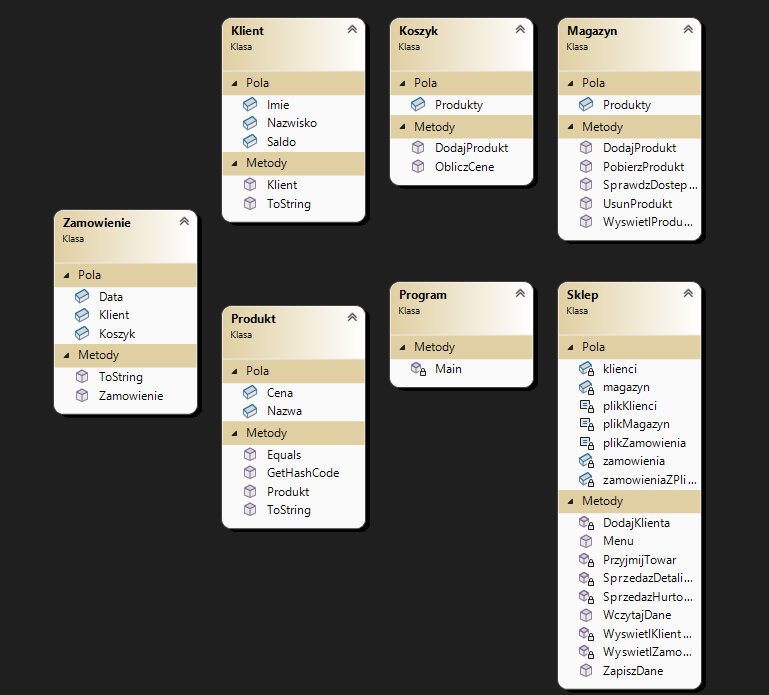
\includegraphics[width=0.9\linewidth]{figures/Hierarchia_klas.png}
    \caption{Diagram klas}
\end{figure}

\section{Zarządzanie danymi i baza danych}
Dane w systemie są przechowywane w trzech głównych plikach tekstowych:
\begin{itemize}
    \item \textbf{magazyn.txt} – zawiera informacje o produktach w formacie: nazwa; cena; ilość,
    \item \textbf{klienci.txt} – przechowuje dane klientów: imię; nazwisko; saldo,
    \item \textbf{zamowienia.txt} – zapisuje historię transakcji, zawierając datę, informacje o kliencie (lub informację o sprzedaży detalicznej) oraz listę zakupionych produktów.
\end{itemize}
Operacje CRUD (tworzenie, odczyt, aktualizacja, usuwanie) są realizowane poprzez odczytywanie danych z powyższych plików przy uruchomieniu systemu oraz zapisywanie zmian po zakończeniu pracy.


% ********** Koniec rozdziału **********

\newpage
\chapter{Harmonogram realizacji projektu}
\section{Diagram Gantta}
Harmonogram prac nad projektem został przedstawiony za pomocą diagramu Gantta, który ilustruje kolejne etapy realizacji:
\begin{figure}[ht]
    \centering
    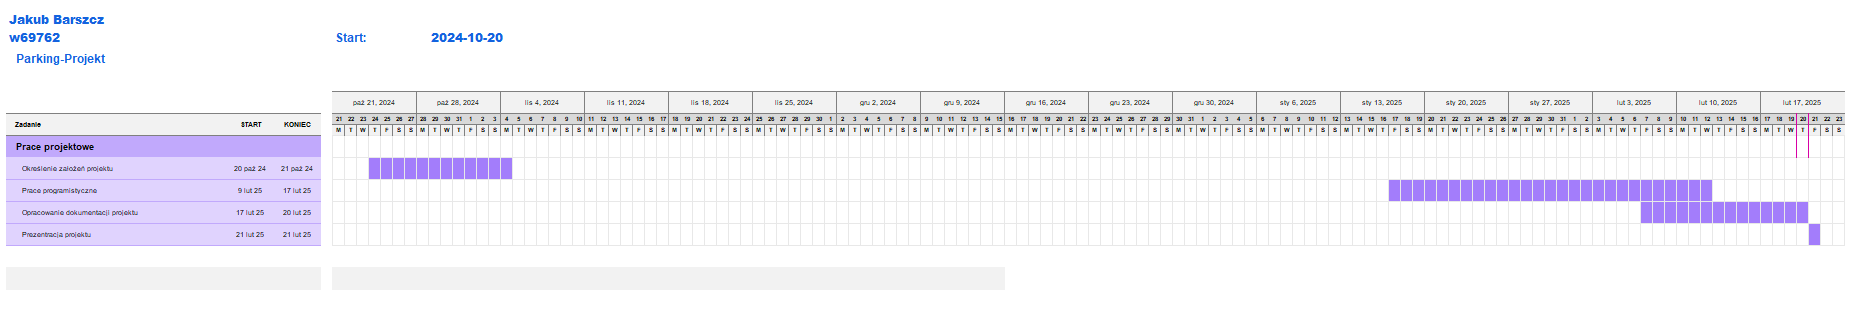
\includegraphics[width=1\linewidth]{figures/Diagram_gantta.png}
    \caption{Diagram Gantta}
\end{figure}

\section{Etapy realizacji}
Projekt został podzielony na następujące etapy:
\begin{itemize}
    \item Określenie założeń projektu
    \item Prace programistyczne
    \item Opracowanie dokumentacji projektu
    \item Prezentacja i obrona projektu
\end{itemize}
\newpage
\chapter{Repozytorium i system kontroli wersji}
\section{Struktura repozytorium}
Kod źródłowy projektu został umieszczony w repozytorium Git, pod następującym linkiem:
\url{https://github.com/JakubBarszcz/Programowanie_Jakub_Barszcz_w69762}

\begin{itemize}
    \item \texttt{/Projekt Programowanie} – katalog zawierający wszystkie pliki źródłowe (np. \texttt{Program.cs}, \texttt{Sklep.cs}, \texttt{Magazyn.cs}, \texttt{Produkt.cs}, \texttt{Koszyk.cs}, \texttt{Klient.cs}, \texttt{Zamowienie.cs}).
    \item \texttt{/Dokumentacja} – katalog zawierający dokumentację projektu oraz pliki graficzne (diagramy).
\end{itemize}

\section{Zarządzanie wersjami}
W projekcie stosowany jest system kontroli wersji Git, co umożliwia:
\begin{itemize}
    \item Regularne commitowanie zmian z krótkimi opisami wprowadzanych modyfikacji.
    \item Pracę z gałęziami (branches) przy dodawaniu nowych funkcjonalności i naprawie błędów.
    \item Integrację zmian przy użyciu pull requests, co umożliwia przegląd i weryfikację kodu przed scałkowaniem z gałęzią główną.
\end{itemize}
% ********** Koniec rozdziału **********

\newpage
\chapter{Prezentacja warstwy użytkowej projektu}
\section{Opis aplikacji}
Aplikacja działa w trybie konsolowym. Po uruchomieniu następuje wczytanie danych z plików tekstowych, a następnie wyświetlenie głównego menu, które umożliwia:
\begin{itemize}
    \item Dodawanie produktów do magazynu,
    \item Realizację sprzedaży detalicznej (z automatycznym obliczaniem wydawanej reszty) oraz hurtowej (dla zarejestrowanych klientów),
    \item Rejestrację nowych klientów,
    \item Wyświetlanie listy produktów, klientów oraz historii zamówień.
\end{itemize}

\section{Przykładowe ekrany}
\subsection{Menu główne}
Widok głównego menu aplikacji. Użytkownik może wybrać jedną z dostępnych opcji: dodawanie produktu do magazynu, sprzedaż (detaliczną lub hurtową), rejestrację nowego klienta, wyświetlenie listy klientów i produktów, a także przegląd zamówień lub wyjście z programu.
\begin{figure}[ht]
    \centering
    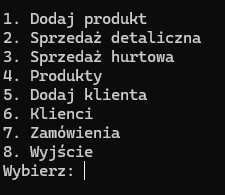
\includegraphics[width=0.5\linewidth]{figures/Menu.png}
    \caption{Menu Główne}
\end{figure}

\subsection{Dodawanie produktu}
Ekran służący do wprowadzania nowego produktu do magazynu. Użytkownik podaje nazwę produktu, cenę oraz ilość. Po poprawnym wprowadzeniu danych wyświetlany jest komunikat potwierdzający dodanie produktu.
\begin{figure}[ht]
    \centering
    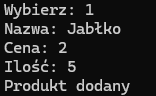
\includegraphics[width=0.5\linewidth]{figures/Dodawanie_pr.png}
    \caption{Dodawanie Produktów}
\end{figure}

\subsection{Sprzedaż detaliczna}
Widok obsługi sprzedaży detalicznej. Użytkownik wybiera produkt na podstawie ID, podaje ilość, a system automatycznie oblicza sumę do zapłaty. Następnie przyjmuje kwotę od klienta i w razie nadpłaty wylicza resztę. Transakcja zostaje zarejestrowana, a stany magazynowe są aktualizowane.
\begin{figure}[ht]
    \centering
    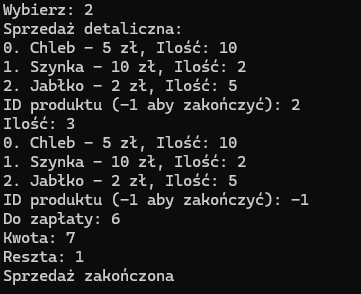
\includegraphics[width=0.5\linewidth]{figures/Spr_det.png}
    \caption{Sprzedaż detaliczna}
\end{figure}

\subsection{Sprzedaż hurtowa}
Ekran realizacji sprzedaży dla zarejestrowanych klientów. Po wprowadzeniu ID klienta, użytkownik wybiera produkty i ich ilości. Kwota za zakupy jest odejmowana od salda klienta, a magazyn zostaje zaktualizowany. Na końcu wyświetlany jest komunikat potwierdzający zakończenie transakcji.
\begin{figure}[ht]
    \centering
    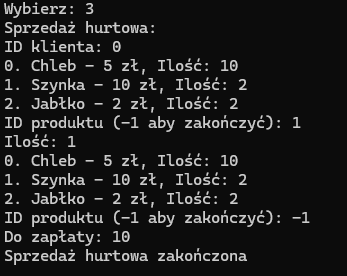
\includegraphics[width=0.5\linewidth]{figures/Spr_hur.png}
    \caption{Sprzedaż hurtowa}
\end{figure}

\subsection{Dodawanie klienta}
Okno pozwalające na dodanie nowego klienta do systemu. Użytkownik podaje imię, nazwisko i saldo portfela. Po wprowadzeniu danych klient jest zapisywany w bazie (plik tekstowy), a aplikacja informuje o poprawnym dodaniu klienta.
\begin{figure}[ht]
    \centering
    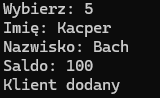
\includegraphics[width=0.5\linewidth]{figures/Dodaj_kl.png}
    \caption{Dodawanie klienta}
\end{figure}

\subsection{Wyświetlanie zamówień}
Widok prezentujący listę zamówień dokonanych w poprzednich sesjach oraz w bieżącej sesji. Każde zamówienie zawiera datę, dane klienta (lub informację o sprzedaży detalicznej), a także listę zakupionych produktów wraz z ich cenami i ilościami. Dzięki temu użytkownik może przejrzeć historię transakcji i sprawdzić szczegóły każdej sprzedaży.
\begin{figure}[ht]
    \centering
    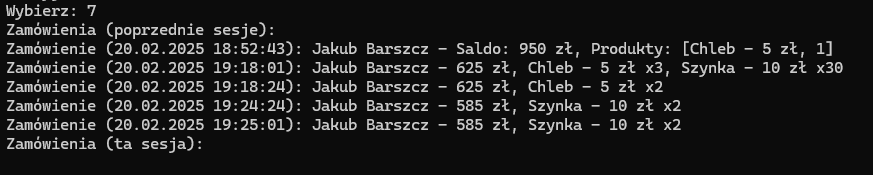
\includegraphics[width=0.9\linewidth]{figures/Zamowienia.png}
    \caption{Wyświetlanie Zamówień}
\end{figure}



\newpage
\chapter{Podsumowanie i dalsze prace rozwojowe}
\section{Podsumowanie}
Projekt „System Zarządzania Sklepem” umożliwia efektywne zarządzanie magazynem, rejestrację klientów oraz realizację sprzedaży w trybie detalicznym i hurtowym. Dzięki zastosowaniu prostych plików tekstowych jako bazy danych, system jest łatwy w implementacji i utrzymaniu. Aplikacja konsolowa stanowi podstawowe narzędzie wspomagające codzienne operacje sklepu, eliminując błędy wynikające z ręcznego prowadzenia dokumentacji oraz przyspieszając procesy decyzyjne.

\section{Planowane dalsze prace}
W przyszłości planowane są:
\begin{itemize}
    \item Rozbudowa modułu raportowania, umożliwiająca generowanie raportów sprzedaży.
    \item Integracja z relacyjną bazą danych w celu zwiększenia skalowalności systemu.
    \item Implementacja graficznego interfejsu użytkownika (GUI) dla poprawy użyteczności.
    \item Rozbudowa funkcjonalności o obsługę zwrotów i program lojalnościowy.
\end{itemize}



% ********** Koniec rozdziału **********
\newpage

% *************** Bibliografia ***************
\begin{thebibliography}{6}
    \item Microsoft, \textit{Dokumentacja C\#}. \url{https://learn.microsoft.com/pl-pl/dotnet/csharp/}
    \item Microsoft, \textit{Dokumentacja platformy .NET}. \url{https://learn.microsoft.com/pl-pl/dotnet/}
    \item Gamma, E., Helm, R., Johnson, R., Vlissides, J., \textit{Design Patterns: Elements of Reusable Object-Oriented Software}. Addison-Wesley.
    \item Dokumentacja narzędzi: Visual Studio, Rider.
\end{thebibliography}

\newpage

% *************** Zakończenie ***************
% *************** Zakończenie ***************

%***************************************************************************************
% W tym miejscu znajdują się polecenia odpowiedzialne za tworzenie
% spisu ilustracji, spisu treści oraz streszczenia pracy
%***************************************************************************************

%spis rysunków
\addcontentsline{toc}{chapter}{Spis rysunków}
\listoffigures
\newpage


% %streszczenie
% \addcontentsline{toc}{chapter}{Streszczenie}
% \noindent
% {\footnotesize{}\textbf{Wyższa Szkoła Informatyki i Zarządzania z siedzibą w Rzeszowie\\
% Kolegium Informatyki Stosowanej}
% \vspace{30pt}

% \begin{center}
% \textbf{Streszczenie pracy dyplomowej inżynierskiej}\\
% \temat
% \end{center}

% \vspace{30pt}
% \noindent
% \textbf{Autor: \autor
% \\Promotor: \promotor
% \\Słowa kluczowe: tutaj umieść słowa kluczowe}
% \vspace{40pt}
% \\Treść streszczenia, czyli kilka zdań dotyczących treści pracy dyplomowej w języku polskim.
% \vspace{80pt}

% \noindent
% \textbf{The University of Information Technology and Management in Rzeszow\\
% Faculty of Applied Information Technology}
% \vspace{30pt}

% \begin{center}
% \textbf{Thesis Summary\\}
% Tytuł pracy w języku angielskim
% \end{center}

% \vspace{30pt}
% \noindent
% \textbf{Author: \autor
% \\Supervisor: \promotor
% \\Key words: tutaj umieść słowa kluczowe}
% \vspace{40pt}
% \\Treść streszczenia, czyli kilka zdań dotyczących treści pracy dyplomowej w języku angielskim - tłumaczenie tekstu z języka polskiego.
% }

% *************** Koniec pliku back.tex ***************


\end{document}
% *************** Koniec pliku szablon.tex ***************
